\documentclass[mathserif,10pt]{beamer}
\usepackage{amsmath}
\usepackage{amsfonts}
\usepackage{amssymb}
\usepackage{bm}
\usepackage{caption}
\usepackage[normalem]{ulem}
\captionsetup{justification=justified}
\usepackage{eulervm}

\mode<presentation>
{
  \usetheme{default}
  \usecolortheme{default}
  \usefonttheme{default}
  \setbeamertemplate{navigation symbols}{}
  \setbeamertemplate{caption}[numbered]
}

\usepackage[english]{babel}
\usepackage[utf8x]{inputenc}

\title{\large \emph{Semi-supervised classification with graph convolutional networks} by Kipf and Welling}

\author{\scriptsize Samuel Unicomb}
\institute{\scriptsize MACSI, Department of Mathematics and Statistics, University of Limerick}

\date{\scriptsize \today}
%\date{\scriptsize November 20, 2023}

\addtobeamertemplate{navigation symbols}{}{%
  \usebeamerfont{footline}%
  \usebeamercolor[gray]{footline}%
  \hspace{1em}%
  \insertframenumber/\inserttotalframenumber
}

\begin{document}

\def\fontspec{\fontsize{9pt}{11}\selectfont}

\begin{frame}
	\titlepage
\end{frame}

\section{Introduction}

\begin{frame}
  Node representations $H^{(l)}$ are embedded recursively following
  \begin{equation}
    H^{(l + 1)} = \sigma\left(W^{(l)} H^{(l)} \hat{A} \right),
  \end{equation}
  where
  \begin{itemize}
    \item[1.] column $i$ of $H^{(l)}$ is the $l$-th embedding $h^{(l)}_i$ of node $i$
    \item[2.] $H^{(0)} = X$ where $X$ are graph feature vectors
    \item[3.] $W^{(l)}$ is a matrix of adjustable weights
    \item[4.] $\sigma$ is a nonlinear function such as $\text{ReLU}$ or $\tanh$
    \item[5.] $\hat{A}$ is a symmetrically normalised Laplacian with entries
    \begin{equation*}
      \hat{A}_{ij} = \dfrac{A_{ij} + I_{ij}}{\sqrt{(k_i + 1)(k_j + 1)}}.
    \end{equation*}
  \end{itemize}
\end{frame}

\begin{frame}
%  Equation (9) of main text transforms $X$ as
  \begin{subequations}
     \begin{align}
        H^{(0)} &= X \\
        M^{(0)} &= H^{(0)}\hat{A} \\
        H^{(1)} &= \text{ReLU}\left(W^{(0)} M^{(0)}\right) \\
        M^{(1)} &= H^{(1)}\hat{A} \\
        H^{(2)} &= \text{softmax}\left(W^{(1)} M^{(1)}\right)
     \end{align}
  \end{subequations}
\end{frame}

\begin{frame}
  \begin{figure}
    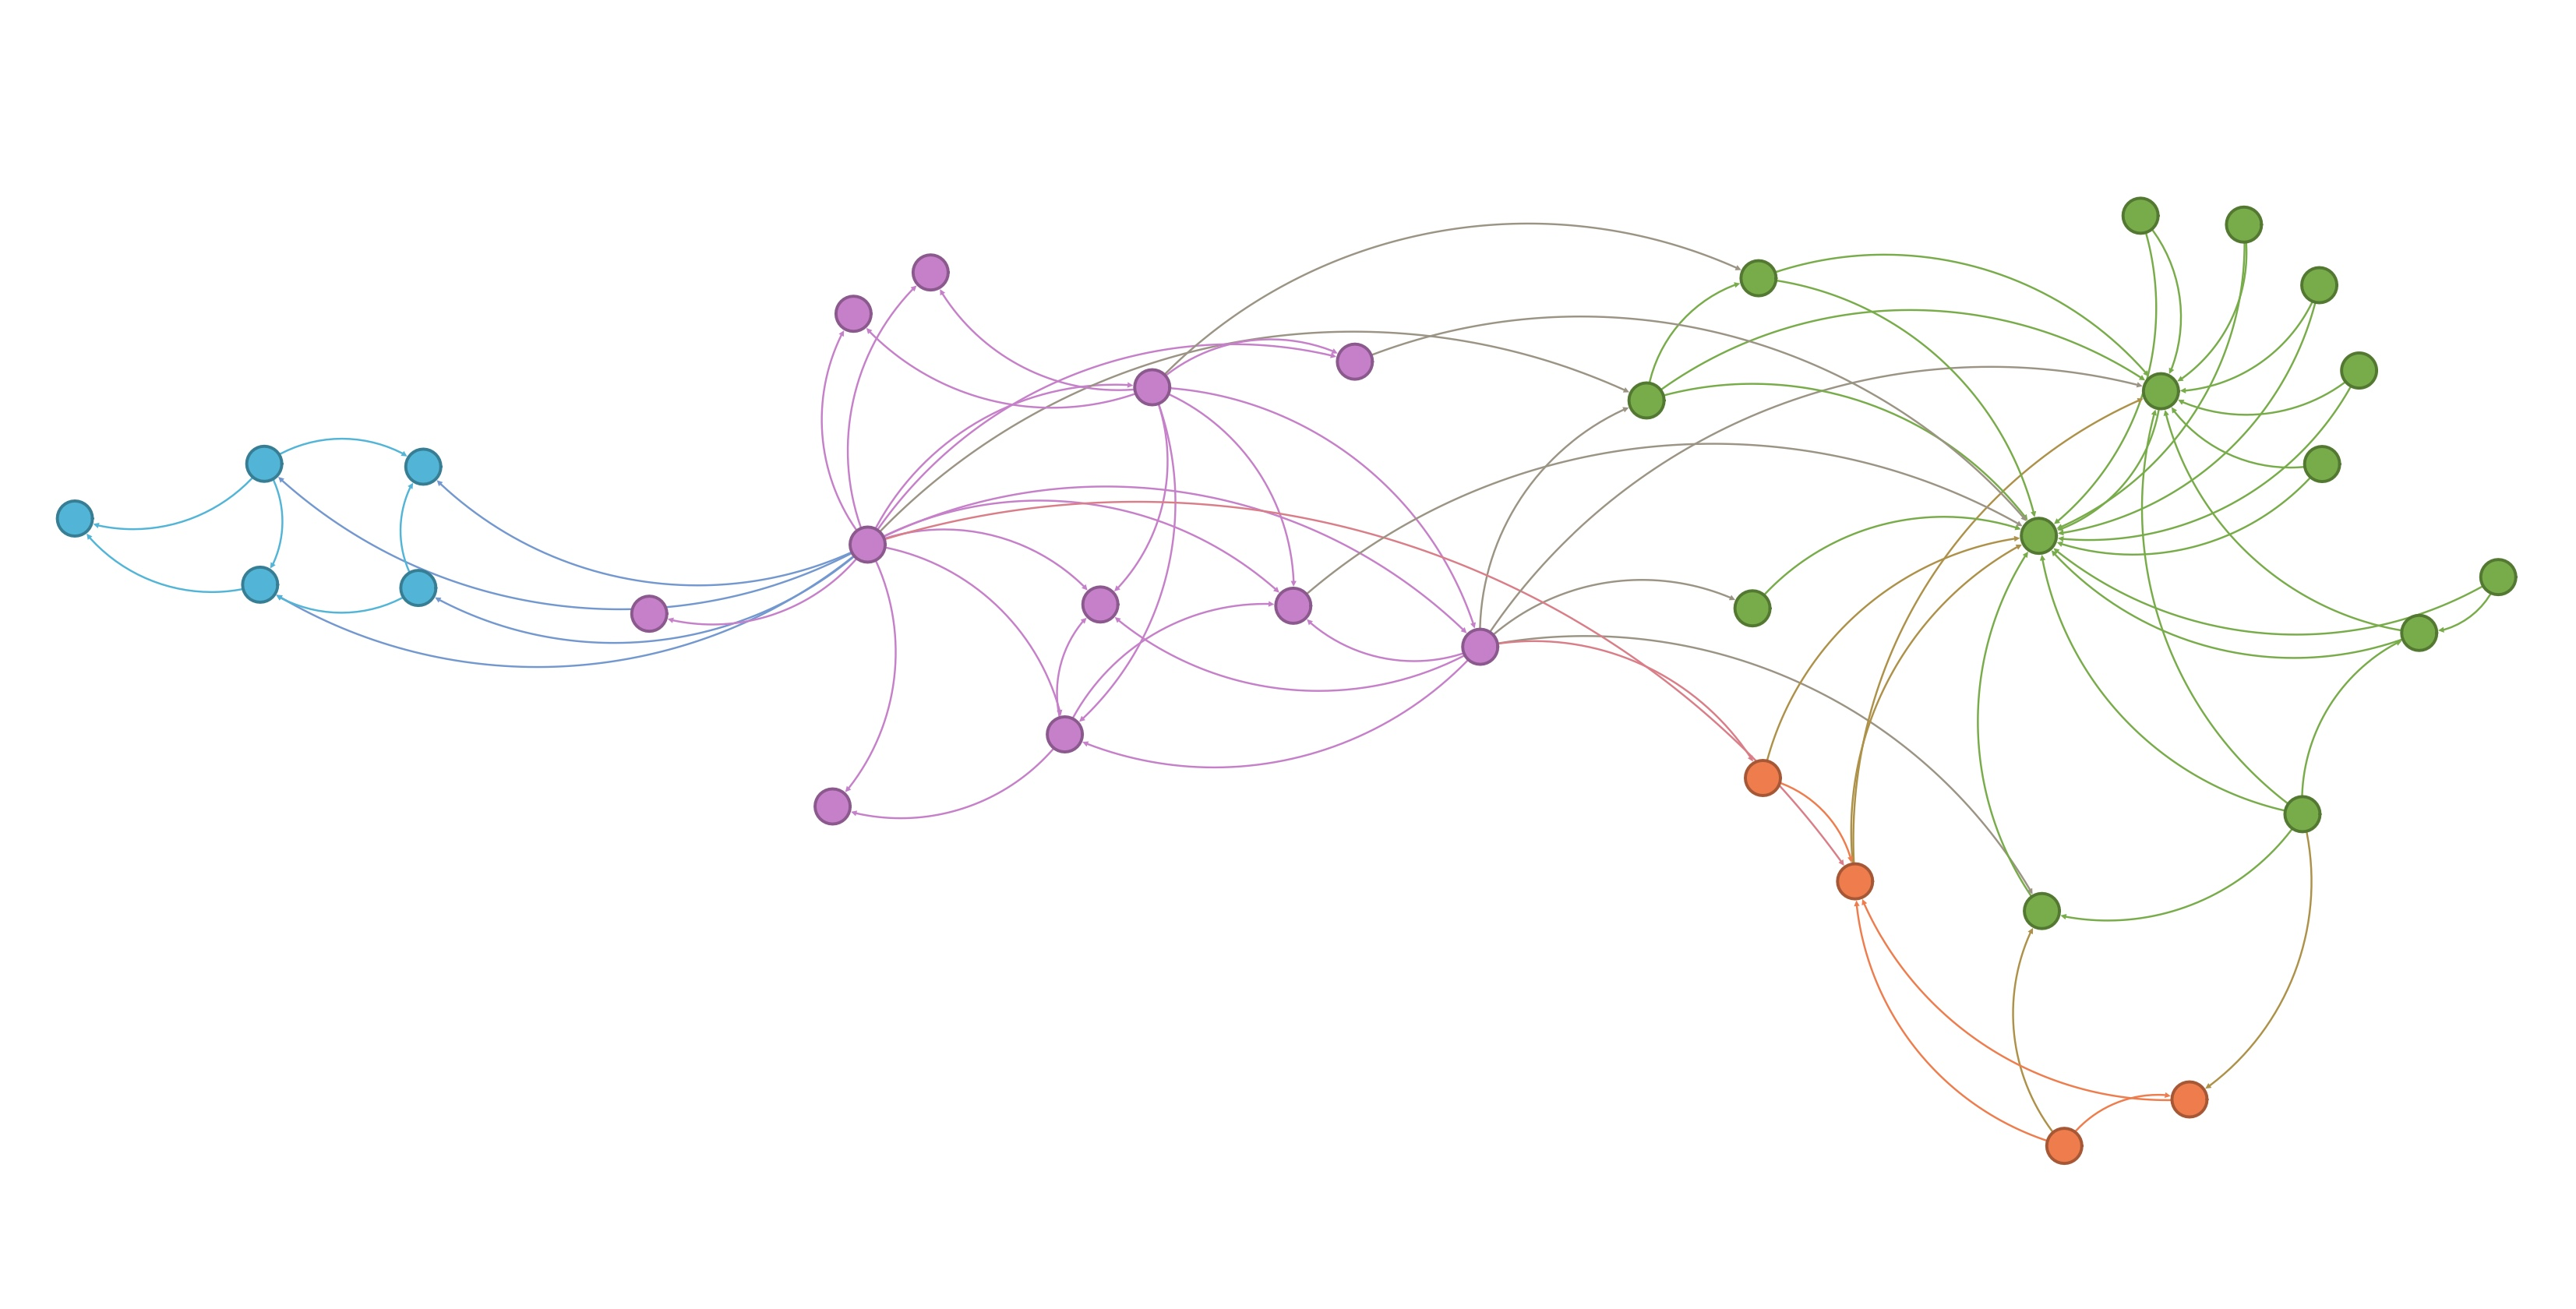
\includegraphics[scale=0.09]{figs/zachary.jpg}
    \caption{Zachary karate club coloured using Louvain method in \emph{Gephi}.}
  \end{figure}
\end{frame}

\begin{frame}
  \begin{subequations}
    \begin{align}
      H^{(0)} &= X \\
      M^{(0)} &= H^{(0)}\hat{A} \\
      H^{(1)} &= \tanh \left(W^{(0)} M^{(0)}\right) \\
      M^{(1)} &= H^{(1)}\hat{A} \\
      H^{(2)} &= \tanh \left(W^{(1)} M^{(1)}\right) \\
      M^{(2)} &= H^{(2)}\hat{A} \\
      H^{(3)} &= \tanh \left(W^{(2)} M^{(2)}\right) \\
      M^{(3)} &= H^{(3)}\hat{A} \\
  Z = H^{(4)} &= \text{softmax}\left(W^{(4)} M^{(4)}\right)
    \end{align}
  \end{subequations} 
\end{frame}

\begin{frame}
  \begin{figure}
    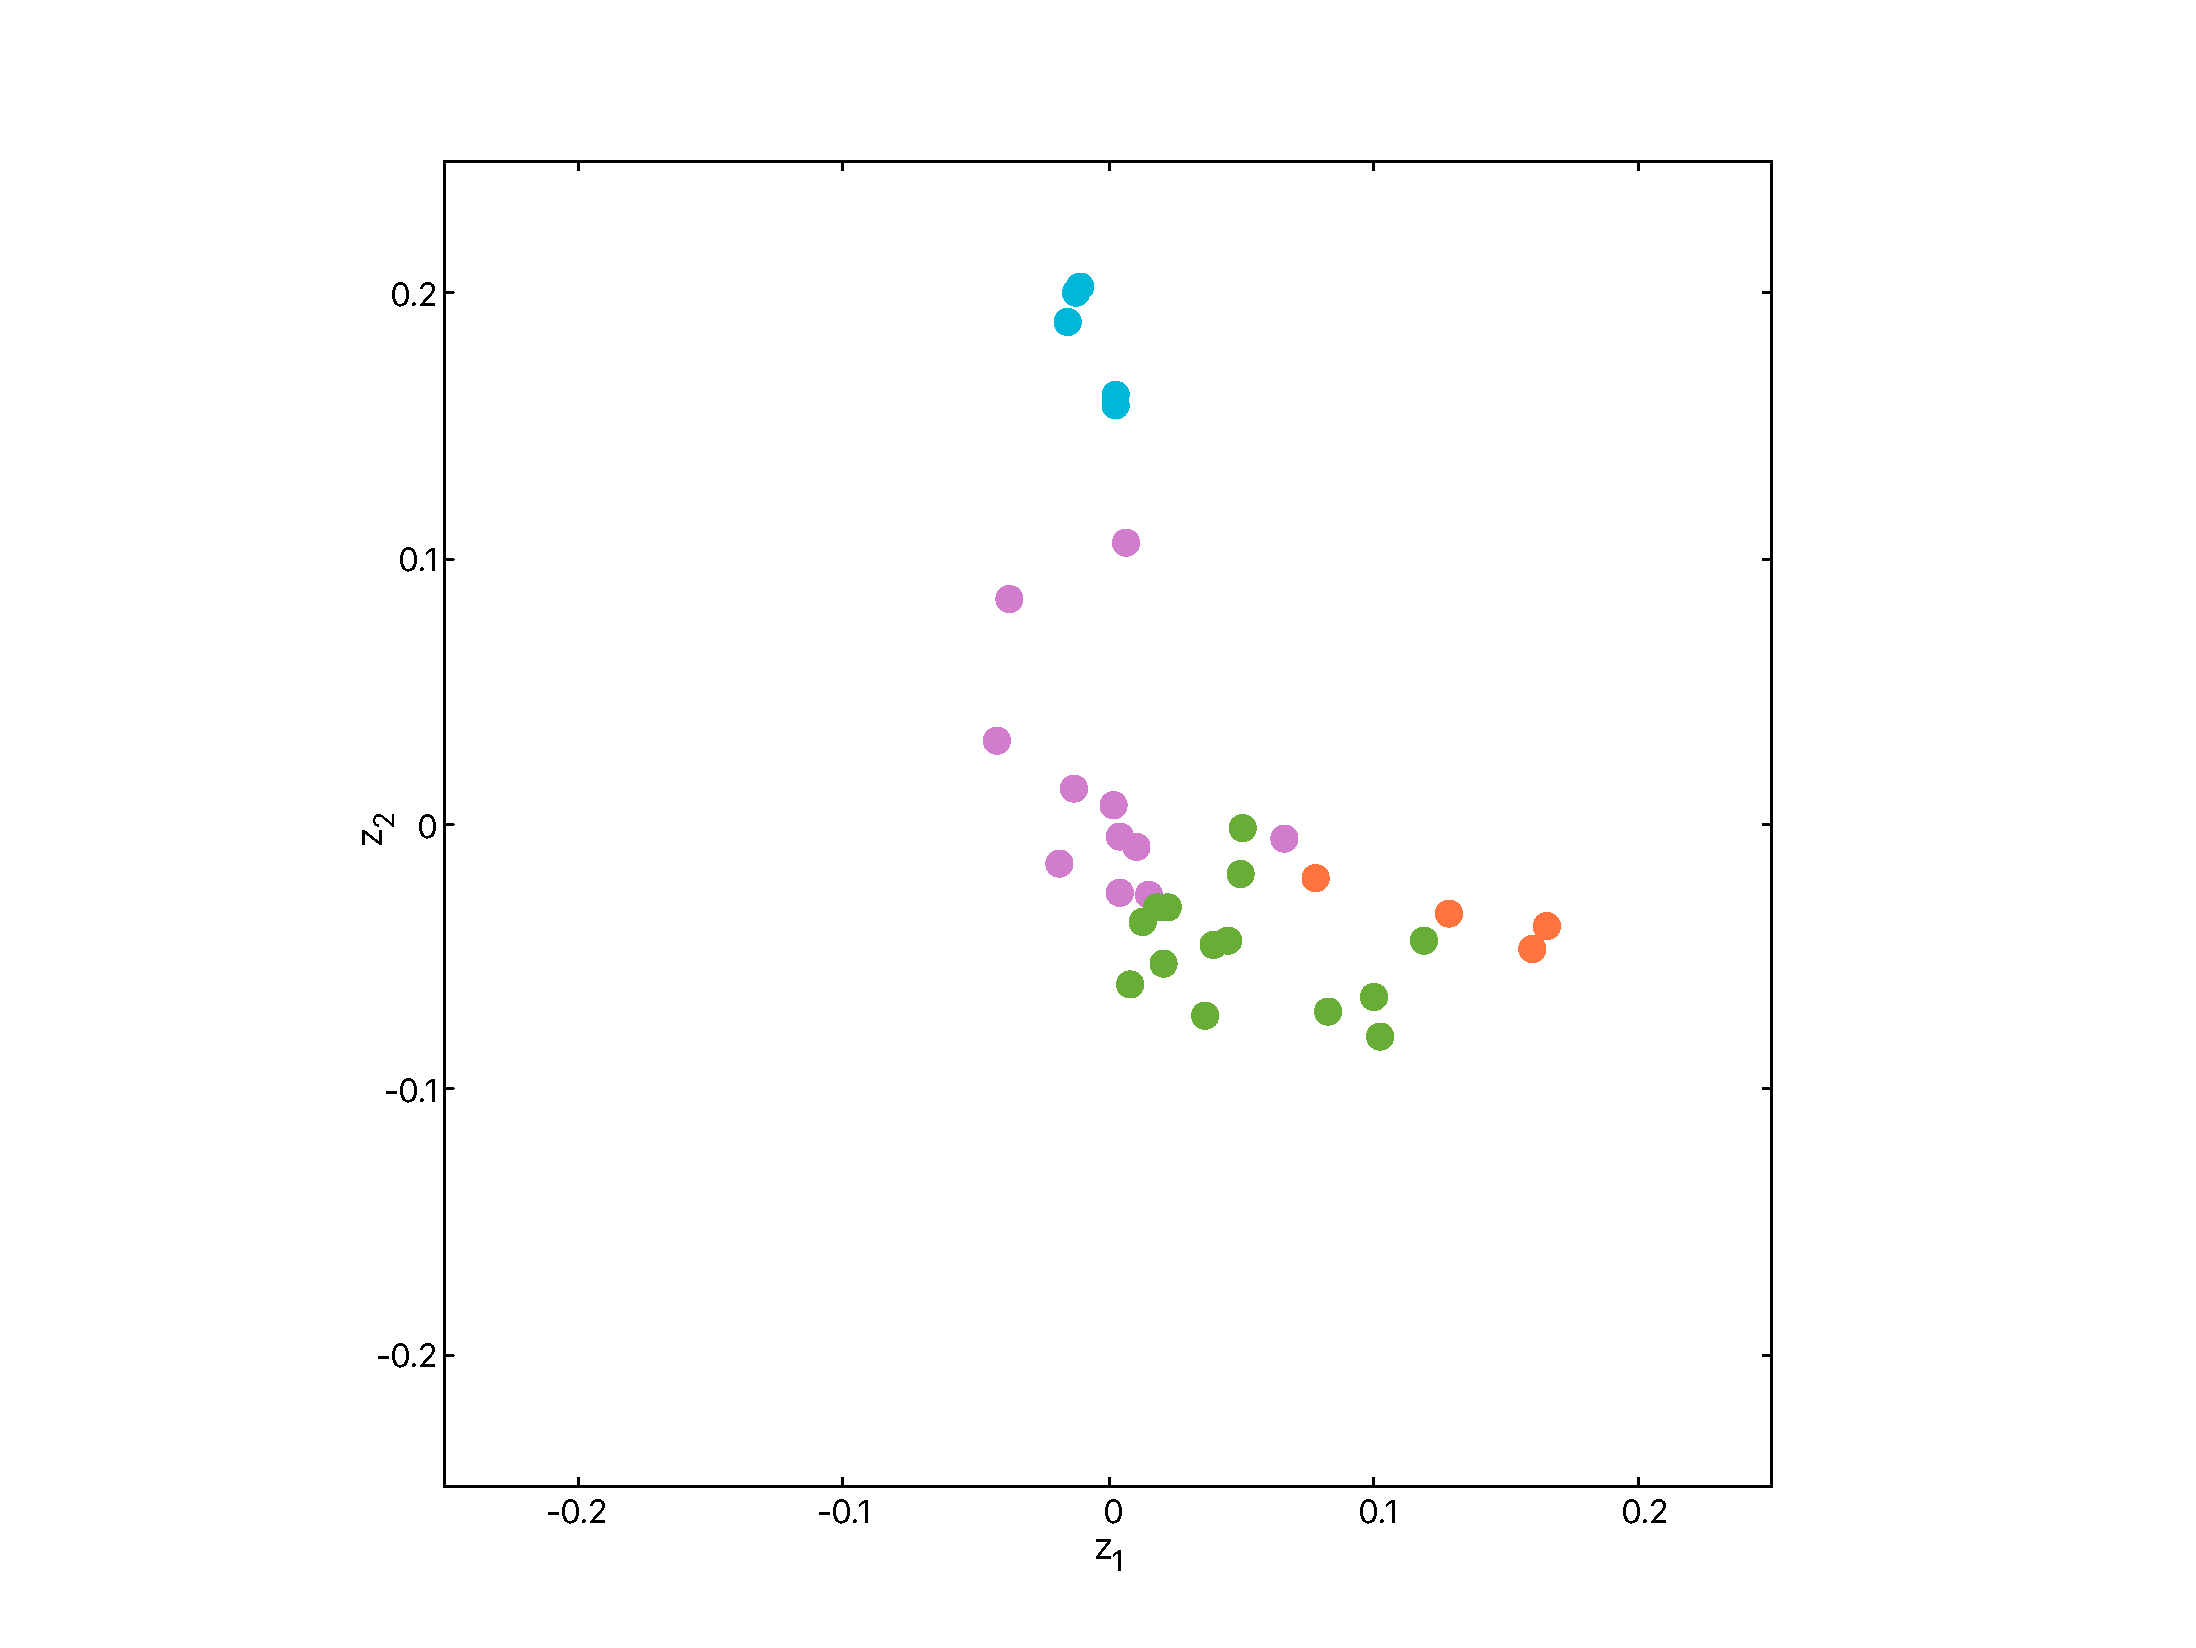
\includegraphics[scale=0.25]{figs/fig01b.pdf}
    \caption{Unsupervised embedding of Zachary karate club.}
  \end{figure}
\end{frame}

\begin{frame}
  \begin{figure}
    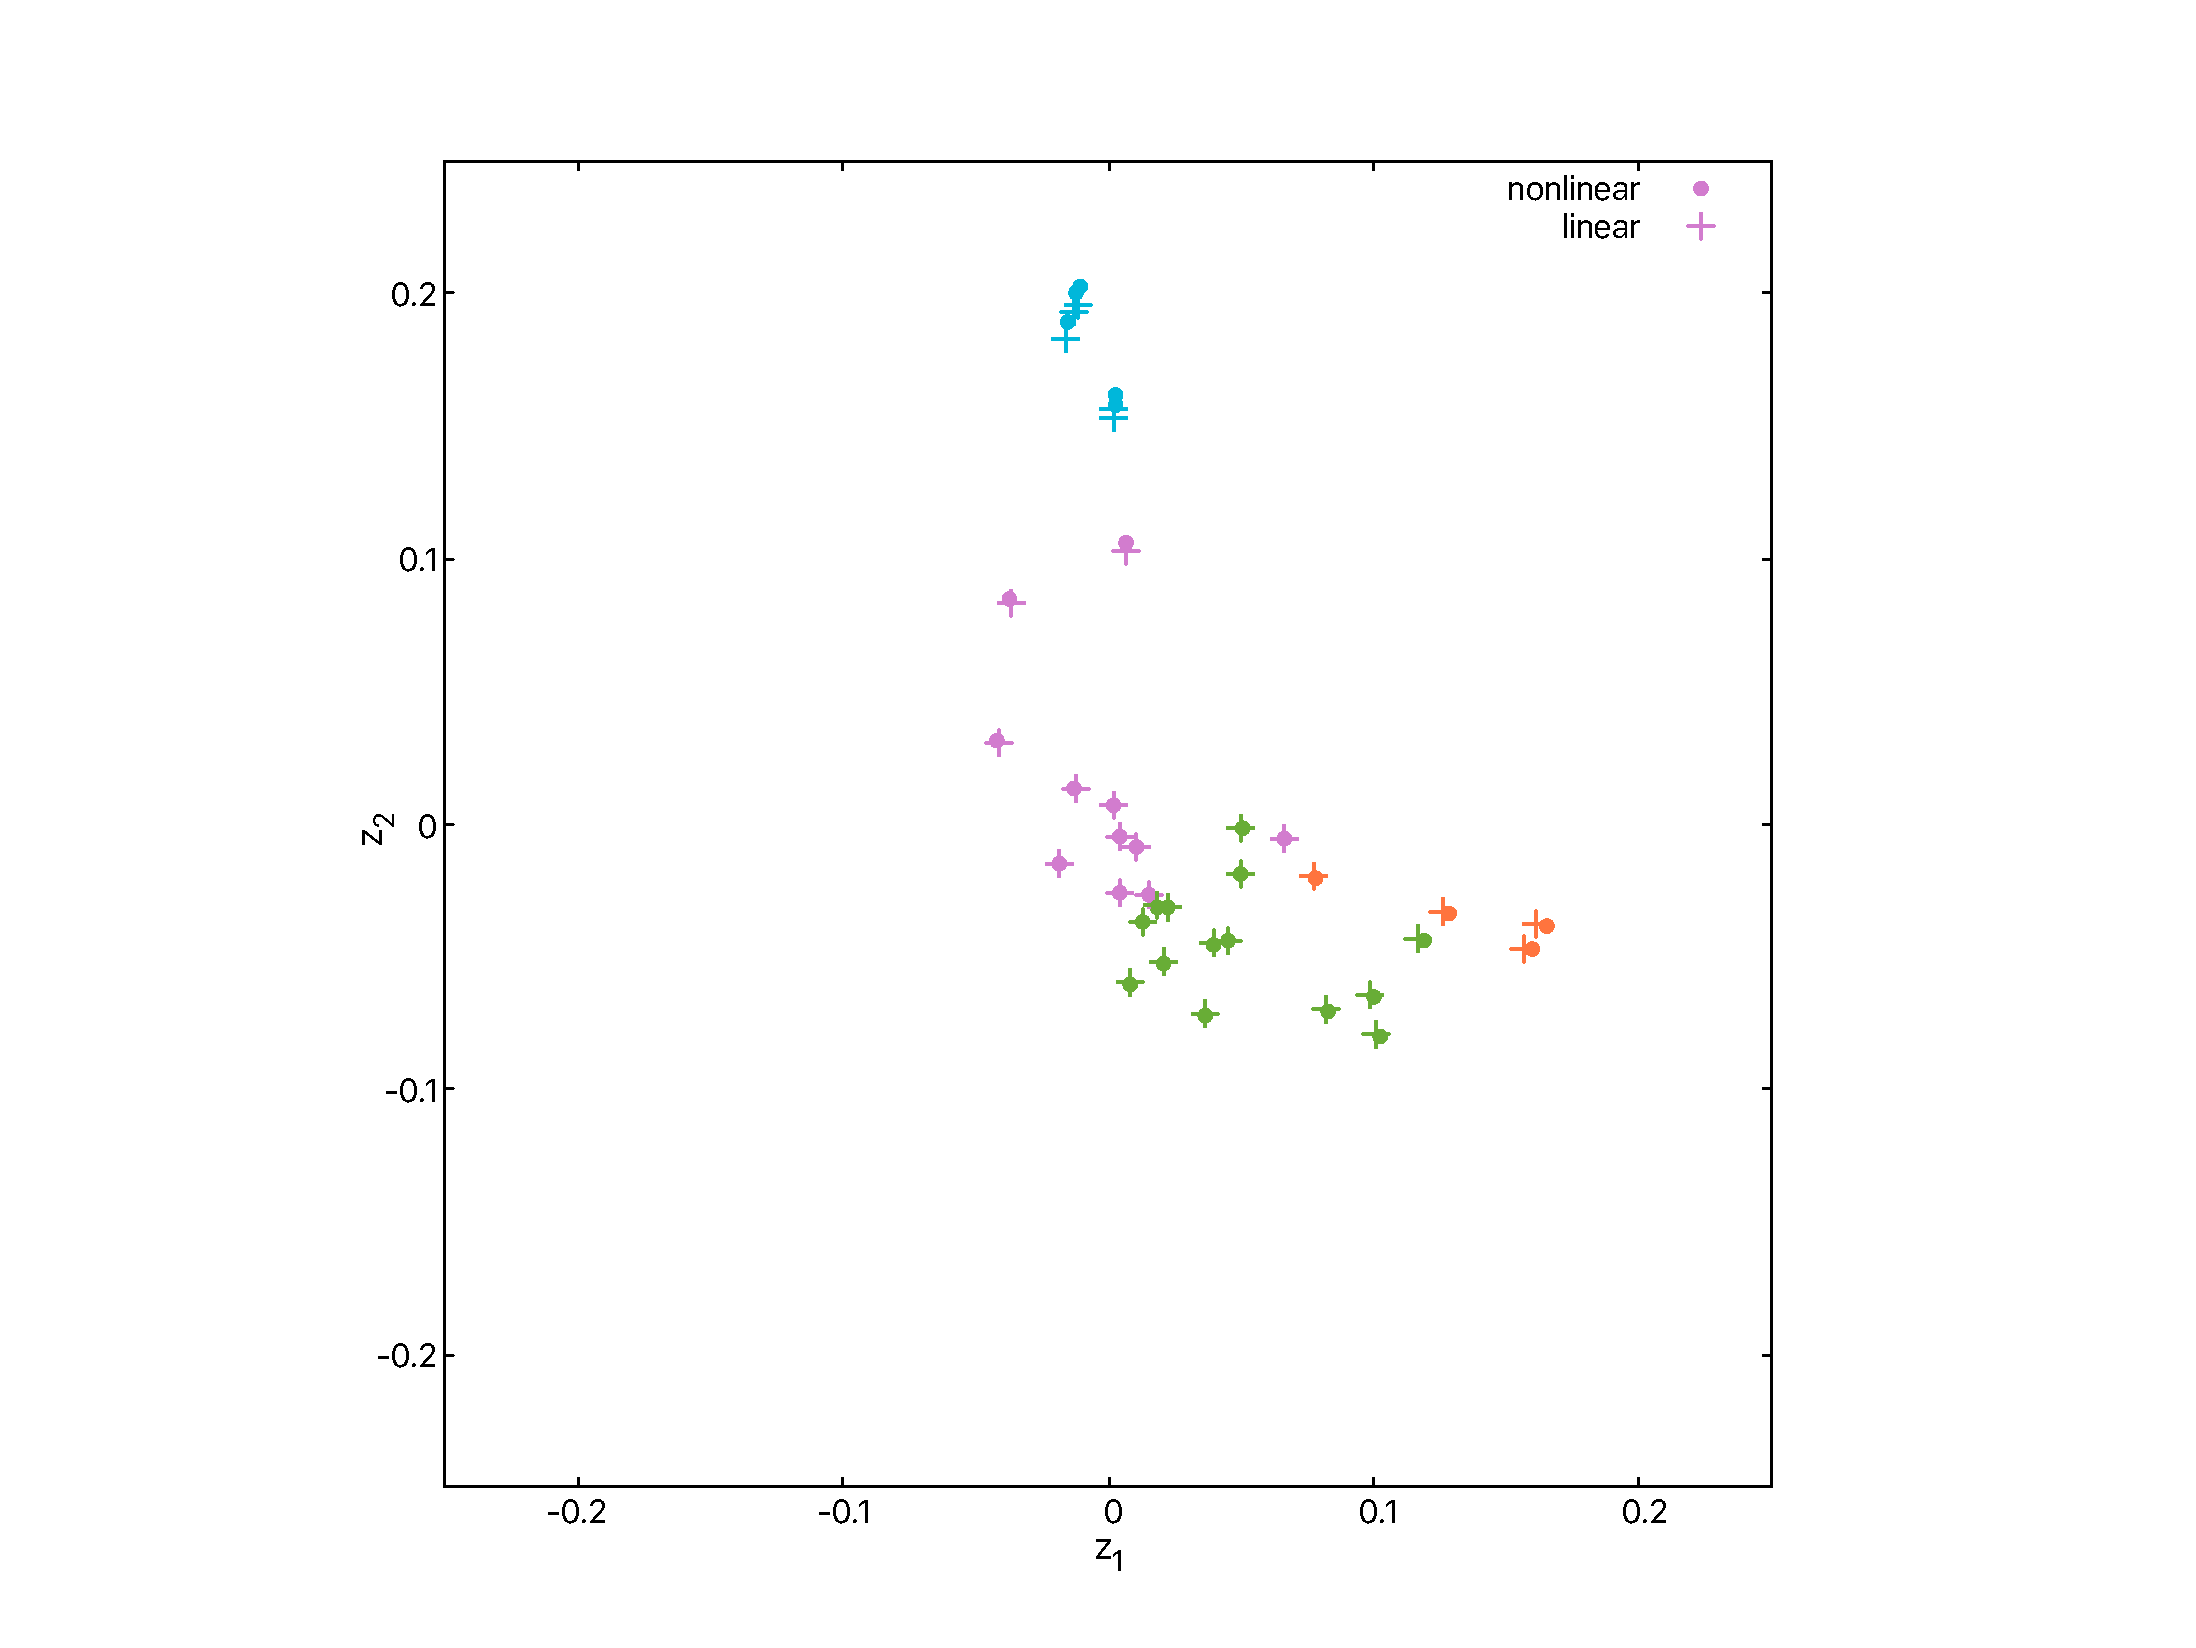
\includegraphics[scale=0.25]{figs/fig01c.pdf}
    \caption{Comparing $\sigma(\tilde{H}^{(l)}) = \tanh(\tilde{H}^{(l)})$ and $\text{id}(\tilde{H}^{(l)})$.}
  \end{figure}
\end{frame}

\begin{frame}
We add a softmax layer and apply the cross-entropy loss
\begin{equation}
  \mathcal{L} = -\sum_{l \in \mathcal{Y}_L} \sum_f Y_{fl} \ln Z_{fl}
\end{equation}
where 
\begin{itemize}
  \item[1.] $\mathcal{Y}_L$ contains indices of nodes that are labelled
  \item[2.] $f \in \lbrace 0, 1, 2, 3 \rbrace$ indexes the node classes in Zachary 
  \item[3.] $Y_{fl} \in \lbrace 0, 1\rbrace$ indicates class membership of node $l$
  \item[4.] $Z_{fl} = H^{(4)}_{fl} = \text{softmax}(h_{fl}^{(4)})$ is normalised output data.
\end{itemize}
\end{frame}

\begin{frame}
  \begin{figure}
    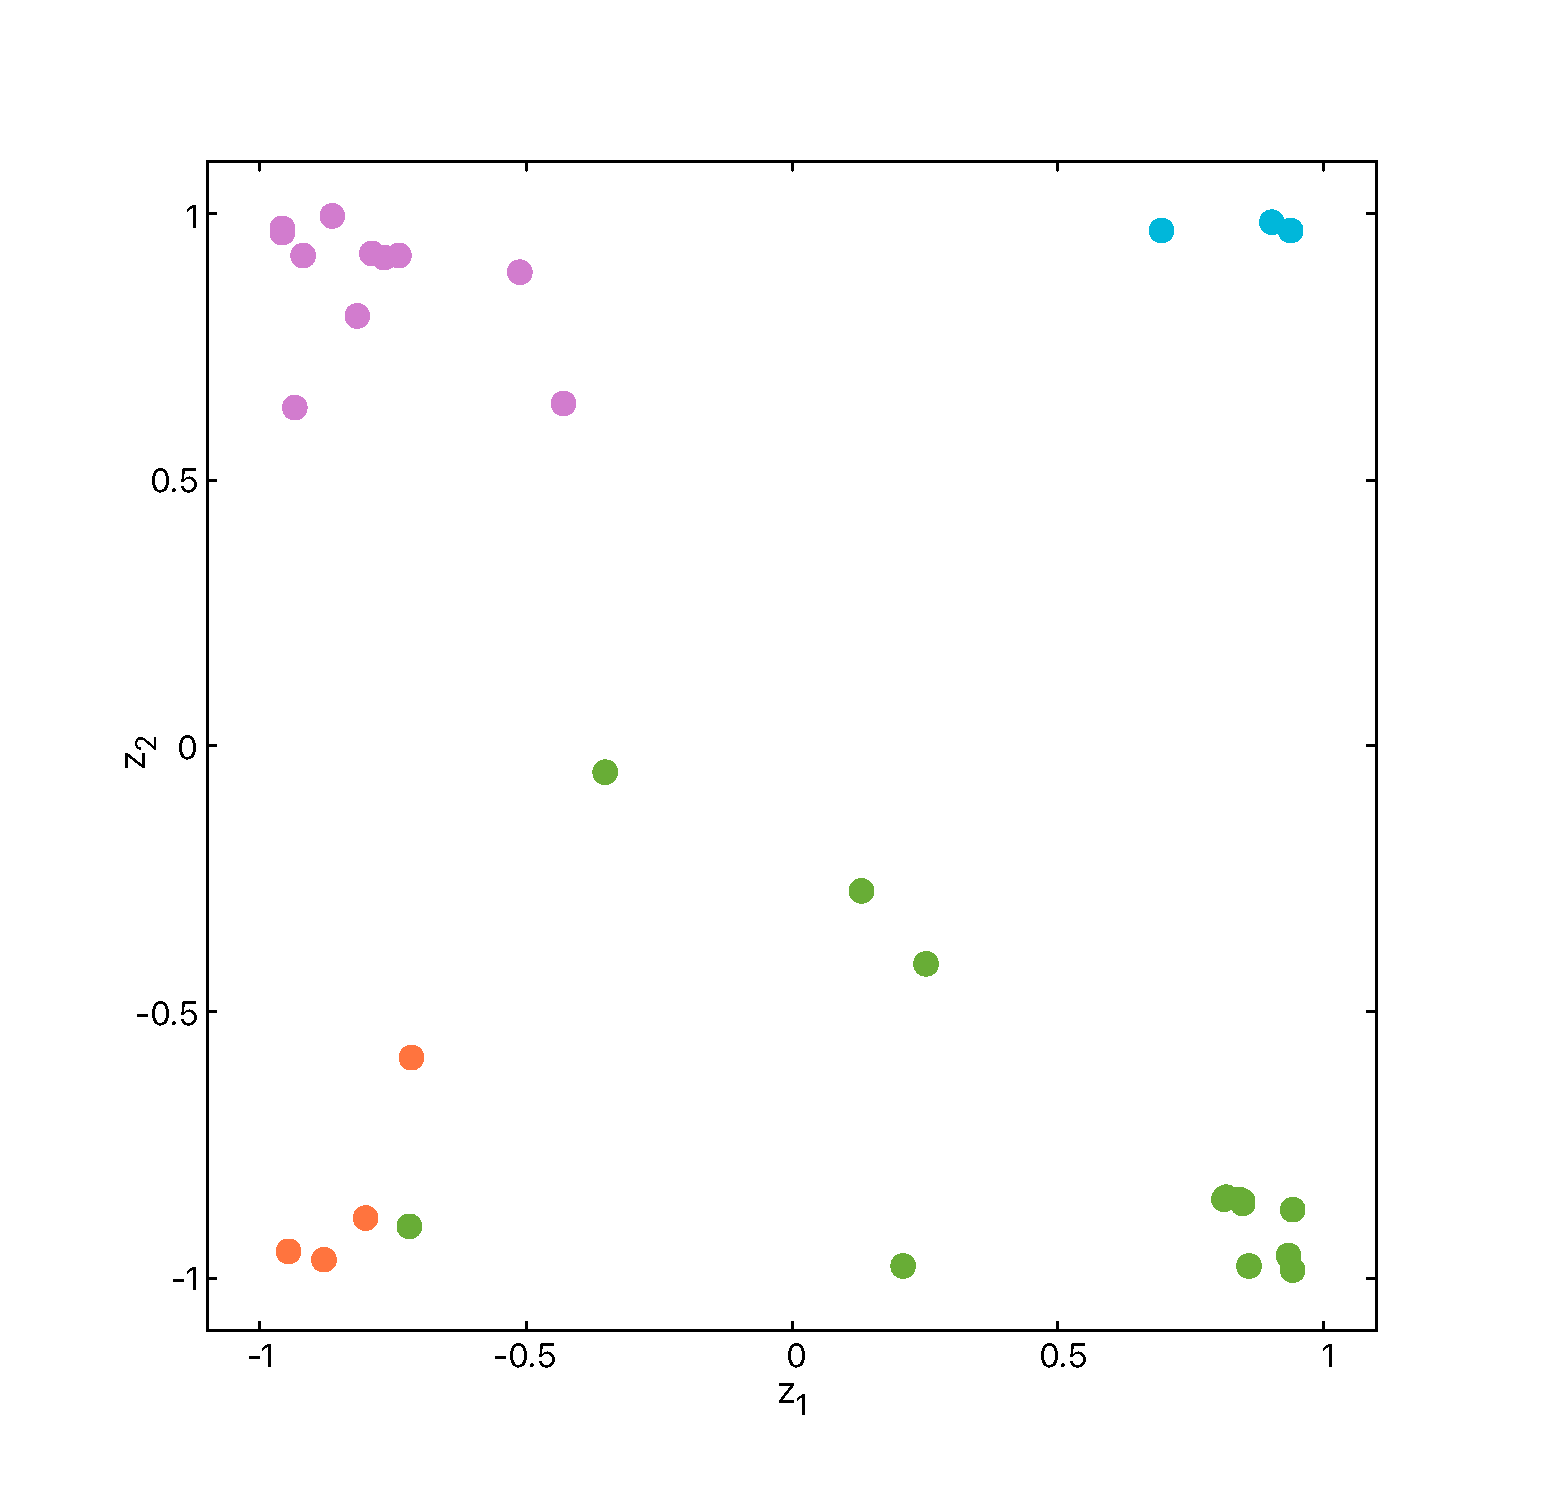
\includegraphics[scale=0.30]{figs/fig02c.pdf}
    \caption{Semi-supervised embedding of Zachary in two dimensions}
  \end{figure}
\end{frame}
  
\begin{frame}
  \begin{figure}
    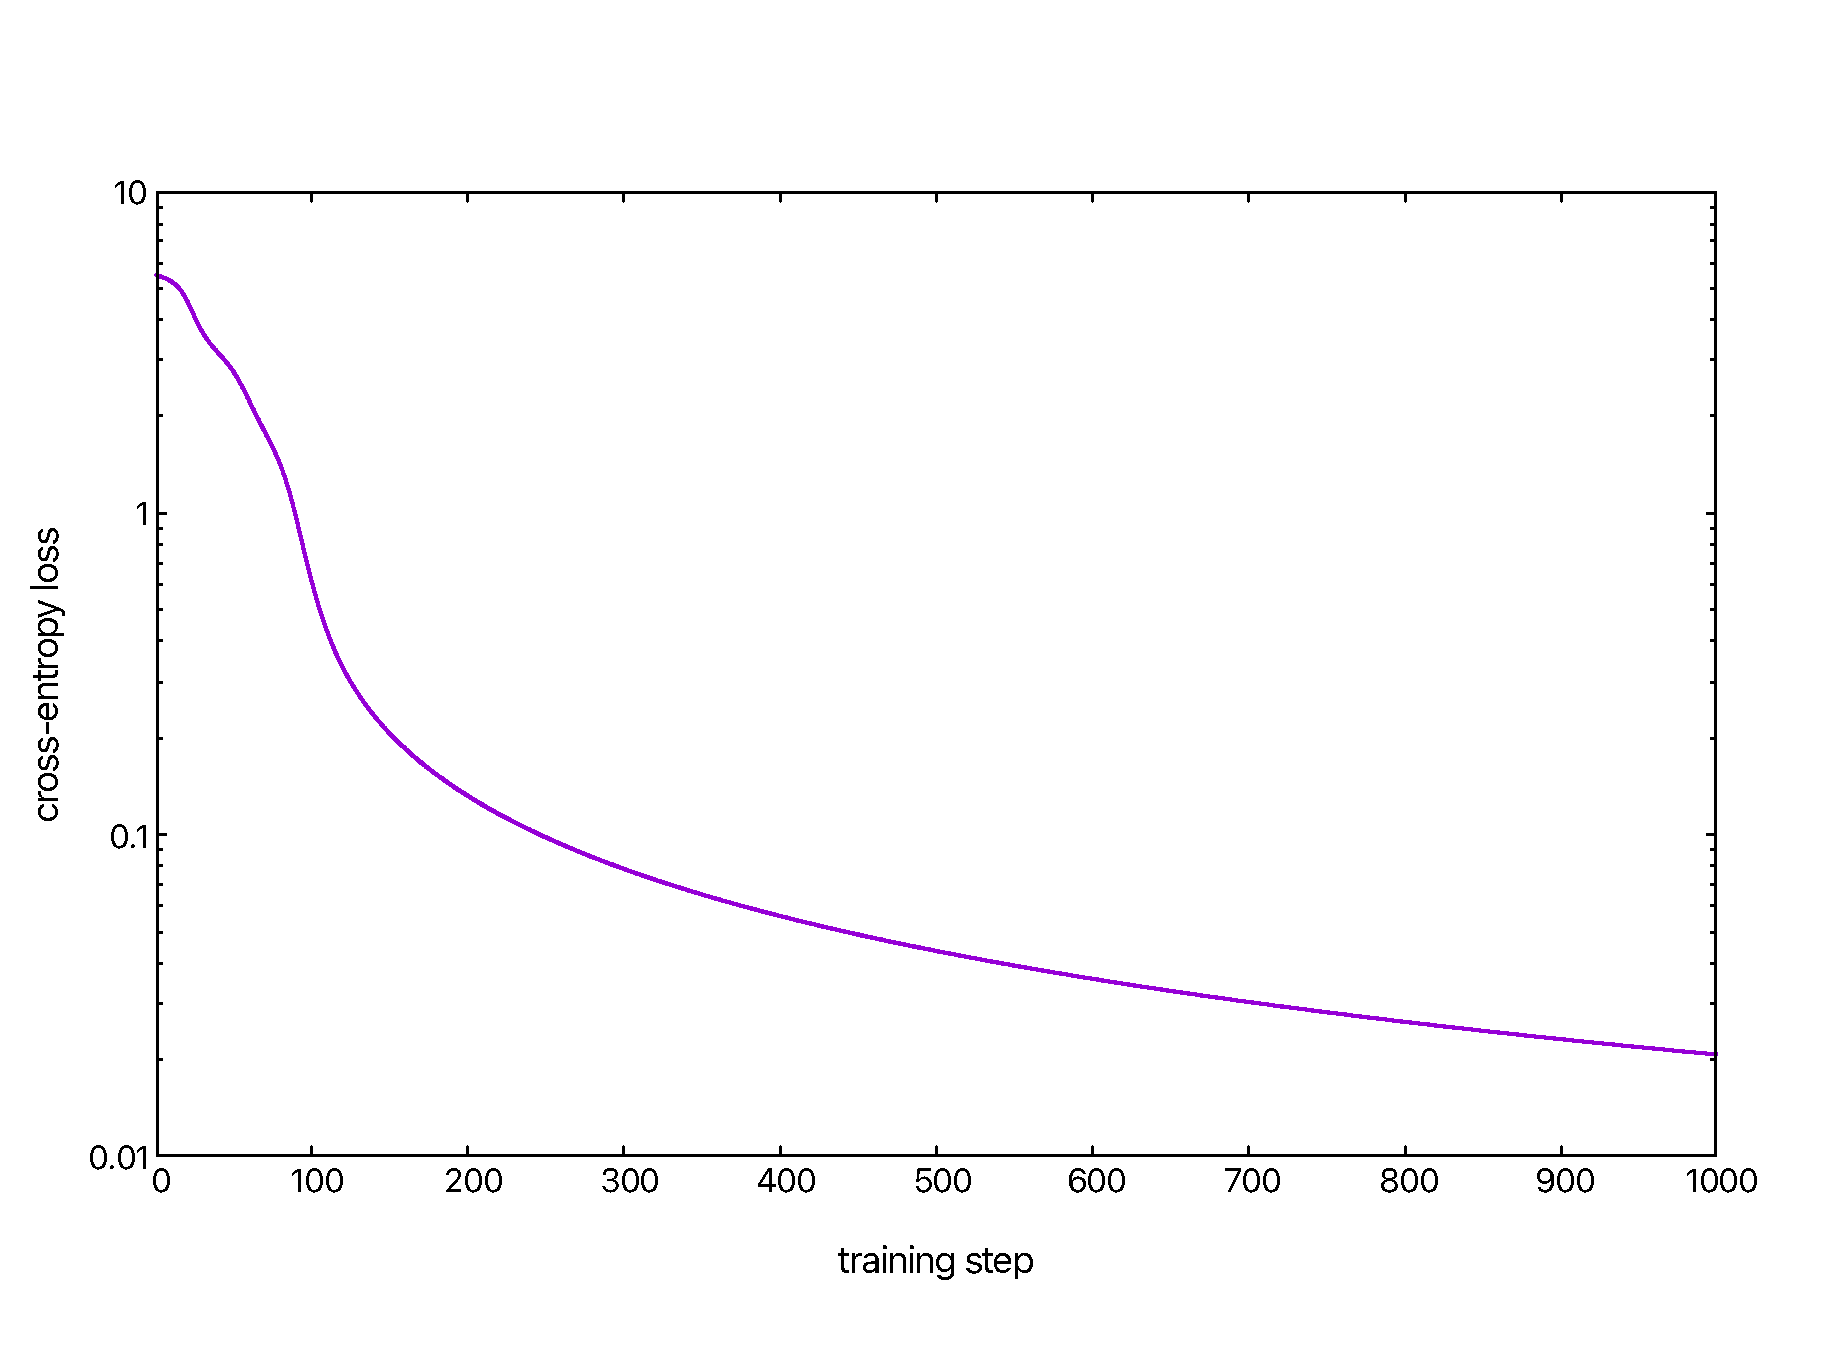
\includegraphics[scale=0.30]{figs/fig02b.pdf}
  \end{figure}
\end{frame}

\begin{frame}
  Change in $\mathcal{L}$ due to a change in $w_{ji}$ is
  \begin{equation}
    \begin{split}
      \dfrac{\partial \mathcal{L}}{\partial w_{ji}} &= \sum_\alpha \dfrac{\partial \mathcal{L}}{\partial h^\alpha_j}\dfrac{\partial h^\alpha_j}{\partial w_{ji}} = \sum_\alpha \delta^\alpha_j m^\alpha_i,
    \end{split}
  \end{equation}
  where $\alpha$ runs over node indices $\lbrace 1, \hdots, |\mathcal{V}|\rbrace$. Then,
  \begin{equation}
    \begin{split}
      \delta^\alpha_j \equiv \dfrac{\partial \mathcal{L}}{\partial h^\alpha_j} =& \sum_k \dfrac{\partial \mathcal{L}}{\partial h^\alpha_k} \dfrac{\partial h^\alpha_k}{\partial h^\alpha_j} + \sum_{\beta} \sum_k \dfrac{\partial \mathcal{L}}{\partial h^\beta_k} \dfrac{\partial h^\beta_k}{\partial h^\alpha_j}\\
      =& \sum_k \delta^\alpha_k \dfrac{\partial h^\alpha_k}{\partial h^\alpha_j} + \sum_{\beta} \sum_k \delta^\beta_k \dfrac{\partial h^\beta_k}{\partial h^\alpha_j}
    \end{split}
  \end{equation}
  where $k$ runs over all cells from $j$, and $\beta \in \text{neighbours}(\alpha)$, with
  \begin{equation}
    \dfrac{\partial h^\alpha_k}{\partial h^\alpha_j} = w_{kj}\dfrac{\sigma^\prime(h_j^\alpha)}{k_\alpha + 1} \quad \text{and} \quad \dfrac{\partial h^\beta_k}{\partial h^\alpha_j} = w_{kj}\dfrac{\sigma^\prime(h_j^\alpha)}{\sqrt{(k_\alpha + 1)(k_\beta + 1)}}.
  \end{equation}
\end{frame}

\begin{frame}
  Compare backpropagation $\nabla \mathcal{L}^{(\text{b})}$ to numerical differentiation $\nabla \mathcal{L}^{(\text{b})}$,
  \begin{equation}
    \dfrac{\partial \mathcal{L}^{(\text{d})}}{\partial w_{ji}} = \dfrac{\mathcal{L}(w_{ji} + \epsilon) - \mathcal{L}(w_{ji} - \epsilon)}{2\epsilon} + \mathcal{O}(\epsilon^2).
  \end{equation}
\end{frame}

\end{document}





